\documentclass[12pt]{article}
\usepackage{hanging}
\usepackage{graphicx}
\usepackage{geometry}
\usepackage{caption}
\usepackage{float}
\usepackage{url}

\captionsetup[figure]{labelfont=it, labelsep=period}

\geometry{left=2cm, right=2cm}

\title{%
  Accuracy of Machine Learning Methods in Predicting Diabetes \\
  \vspace{5mm}
  \large GitHub Repository: https://github.com/alexz957unc/COMP-562-Final-Project}
\author{Alexander Zheng\and Connor Morin\and Jingyu Li\and Yibo Wang}
\date{April 30, 2024}

\begin{document}

\maketitle

\section{Introduction}
According to the CDC, six out of every ten Americans have at least one chronic disease, and among the most prevalent, dangerous, and expensive of them is diabetes (2023a). Diabetes is a chronic disease that affects insulin, a hormone responsible for keeping blood sugar at healthy levels, and it causes the body to either not produce insulin, Type 1, or not respond to it well, Type 2 (CDC, 2023b). The cost and seriousness of diabetes in the U.S. is not to be understated, and it is a problem that continues to worsen. According to the National Diabetes Statistics Report, 38.4 million people in the U.S. have diabetes, diagnosed or undiagnosed, which is over 11 percent of the total population. Furthermore, 97.6 million people have prediabetes, which is a staggering 30 percent of the U.S. population (CDC, 2023c). A 2022 study from the National Library of Medicine estimated the total cost of diabetes to be nearly \$413 billion in both direct medical costs and indirect costs (Parker et al., 2024). 

Unfortunately, the consequences from such statistics are dire. Diabetes serves as a major risk factor for cardiovascular disease, kidney disease, blindness, and many other related diseases and disabilities. As a result, in 2021, the eight leading cause of death in the U.S. was diabetes, with 399,401 death certificates listing diabetes as either an underlying or contributing cause of death (CDC, 2023c). However, this is not all bad news; once an individual learns they have diabetes, certain measures can be taken to mitigate the risks associated with the disease, such as engaging in physical activity and maintaining a healthy diet. This mitigation especially holds true for those with prediabetes and others that may be at risk, as diabetes can be prevented entirely in many cases by taking the appropriate measures.

This notion leads us to some questions that we believe machine learning methods may be particularly useful in answering. If we know that diabetes can be mitigated or prevented, then are there factors which we can use to predict those who may not yet be diagnosed with diabetes but are either undiagnosed or at serious risk? Specifically, can we use ML methods to identify particular risk factors associated with diabetes, and can any of these methods make accurate predictions on if an individual has diabetes? If so, which ML methods are the best and most accurate for doing so? Being able to answer such questions could be the key to helping identify cases of undiagnosed diabetes or individuals that are in danger of developing it so that they can begin to take measures to mitigate or reverse their conditions as soon as possible. These are the questions we look to explore in this analysis.

\subsection{Dataset}
To conduct our analysis, we will be using data from the CDC's Behavioral Risk Factor Surveillance System (BRFSS), which completes yearly telephone surveys for over 400,000 Americans, collecting data about "health-related risk behaviors and events, chronic health conditions, and use of preventive services" (CDC, 2014). The particular dataset we will be using is from a BRFSS survey in 2015, and it contains 70,692 responses and 21 feature variables for each. A response corresponds to an individual with either no diabetes, represented with a "0," or prediabetes or diabetes, represented with a "1," and the dataset contains an even split of responses with no diabetes and prediabetes/diabetes.

\section{Approach}
Our goal is to predict a binary outcome (to be more specific, whether someone has diabetes) using several machine learning classification models. The dataset we used  includes multiple features that could potentially influence the prediction outcome. We have done some processing, such as  encoding categorical variables and splitting the dataset into training and test datasets (80-20 split) for training. 

\subsection{Logistic Regression}
First, using  logistic regression (setting the max iteration to be 2000), we get the following confusion matrix (where the absolute numbers as well as percentages of each category (TP, FP, TN, FN) is presented) and horizontal bar chart that shows the weight of each feature from the dataset that have been used in the Logistic Regression model:
\begin{figure}[H]
  \centering
  \begin{minipage}[b]{0.45\textwidth}
    \centering
    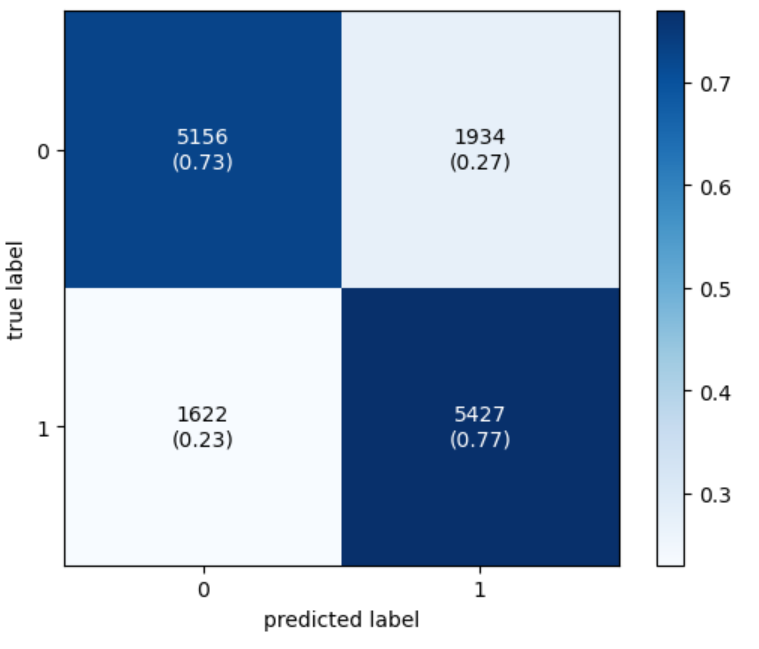
\includegraphics[width=0.7\linewidth]{logreg_cm.png}
    \caption{Logistic Regression confusion matrix}
  \end{minipage}\hfill
  \begin{minipage}[b]{0.45\textwidth}
    \centering
    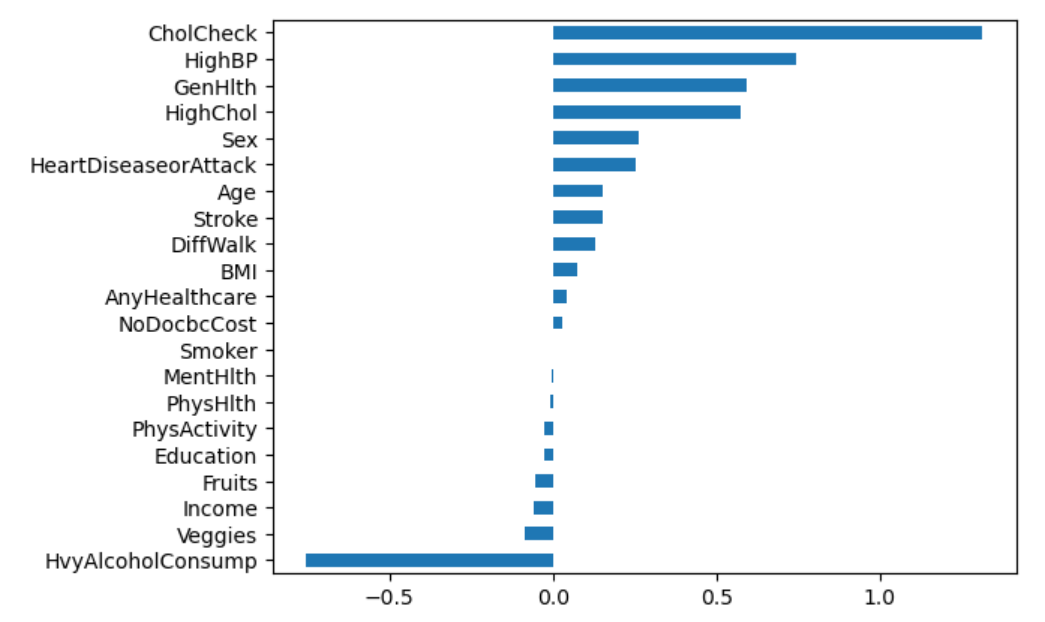
\includegraphics[width=0.7\linewidth]{logreg_w.png}
    \caption{Logistic Regression feature importance}
  \end{minipage}
\end{figure}

\subsection{Decision Tree Classifier}
Second, we tried another approach — Decision Tree Classifier. In this Decision Tree Classifier model, we instantiate the maximum depth of the tree limited to 12 and, similarly, get the following confusion matrix and parameter weight graph:
\begin{figure}[H]
  \centering
  \begin{minipage}[b]{0.45\textwidth}
    \centering
    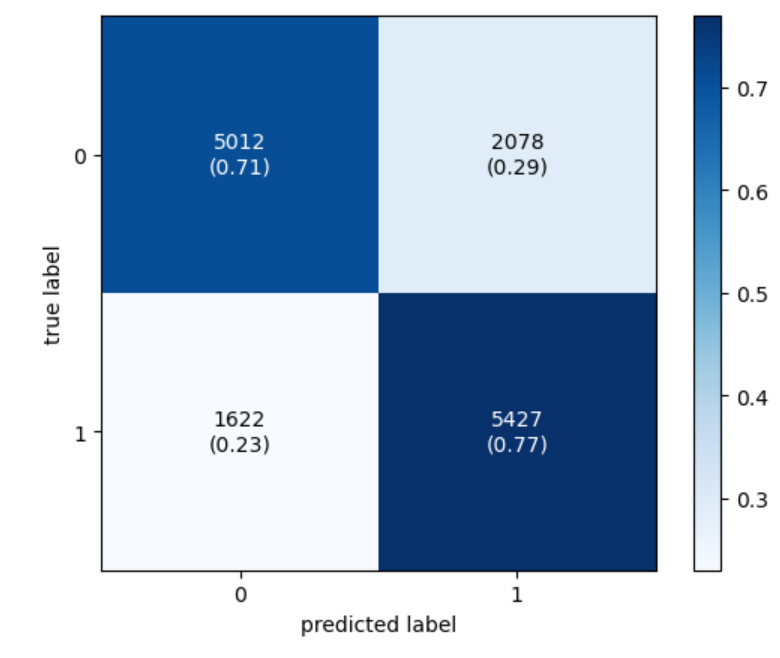
\includegraphics[width=0.7\linewidth]{dectree_cm.png}
    \caption{Decision Tree confusion matrix}
  \end{minipage}\hfill
  \begin{minipage}[b]{0.45\textwidth}
    \centering
    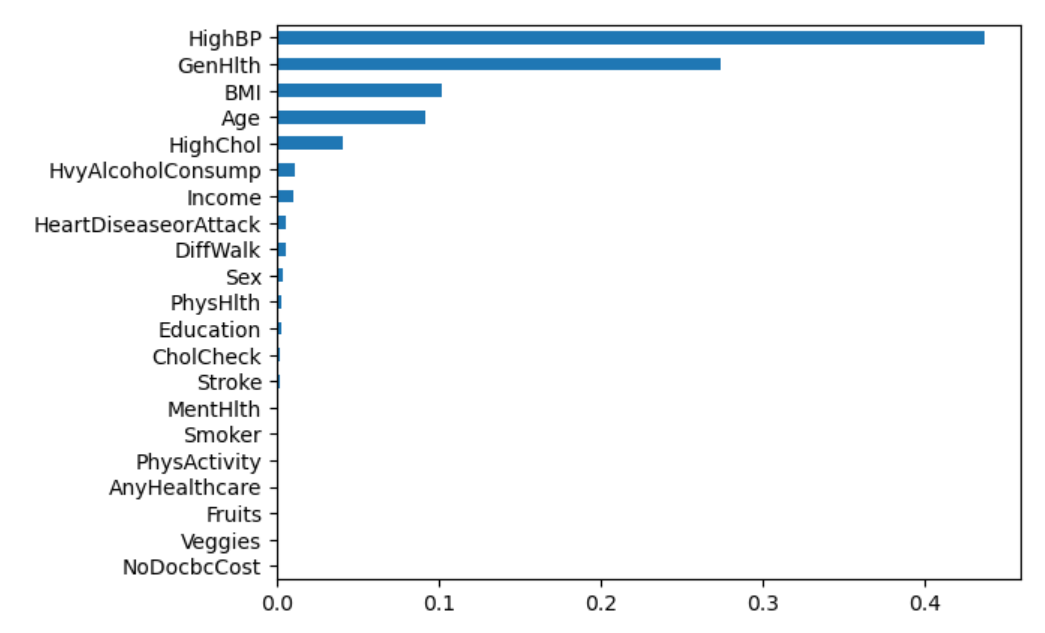
\includegraphics[width=0.7\linewidth]{dectree_w.png}
    \caption{Decision Tree feature importance}
  \end{minipage}
\end{figure}

\subsection{Random Forest}
Third, we use a random forest model. In this random forest model, we set the maximum depth of each tree in the forest to be 12, the number of trees in the forest to be 15, random states to be 42, and get the following confusion matrix and parameter weight graph:
\begin{figure}[H]
  \centering
  \begin{minipage}[b]{0.45\textwidth}
    \centering
    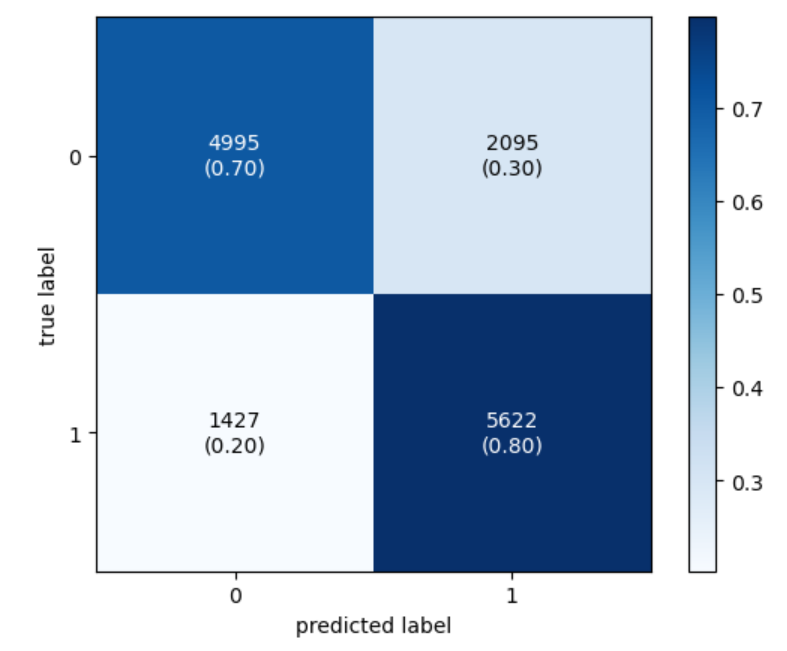
\includegraphics[width=0.7\linewidth]{ranfor_cm.png}
    \caption{Random Forest confusion matrix}
  \end{minipage}\hfill
  \begin{minipage}[b]{0.45\textwidth}
    \centering
    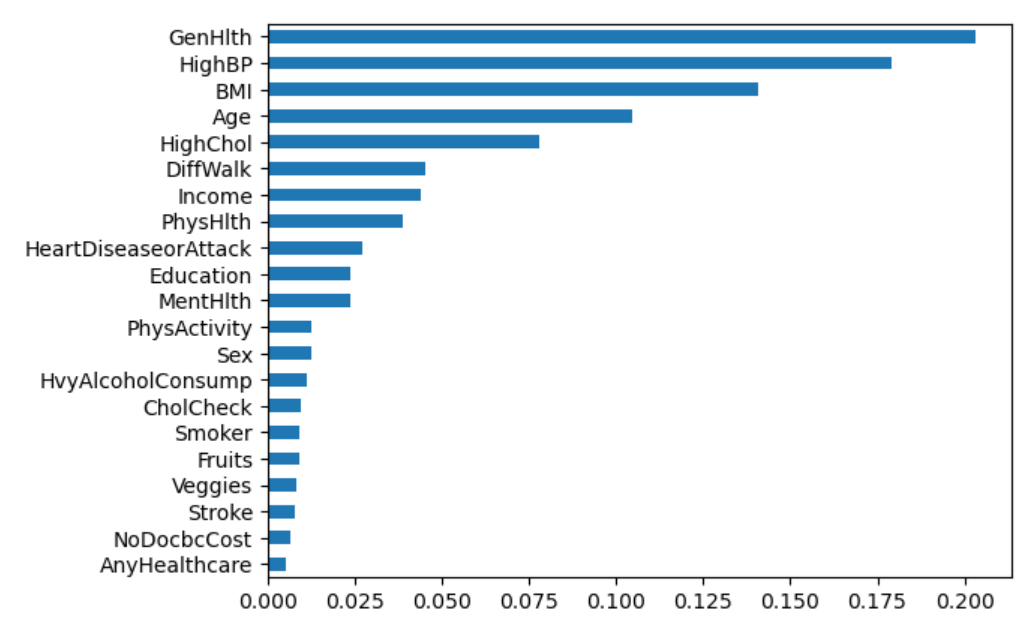
\includegraphics[width=0.7\linewidth]{ranfor_w.png}
    \caption{Random Forest feature importance}
  \end{minipage}
\end{figure}

\subsection{KNN}
Next, we attempted to classify the data with a k-nearest neighbors classifier. The number of neighbors used was determined by taking the square root of the number of total samples. The resulting confusion matrix is below (note that feature importance is not available for KNN).
\begin{figure}[H]
  \centering
  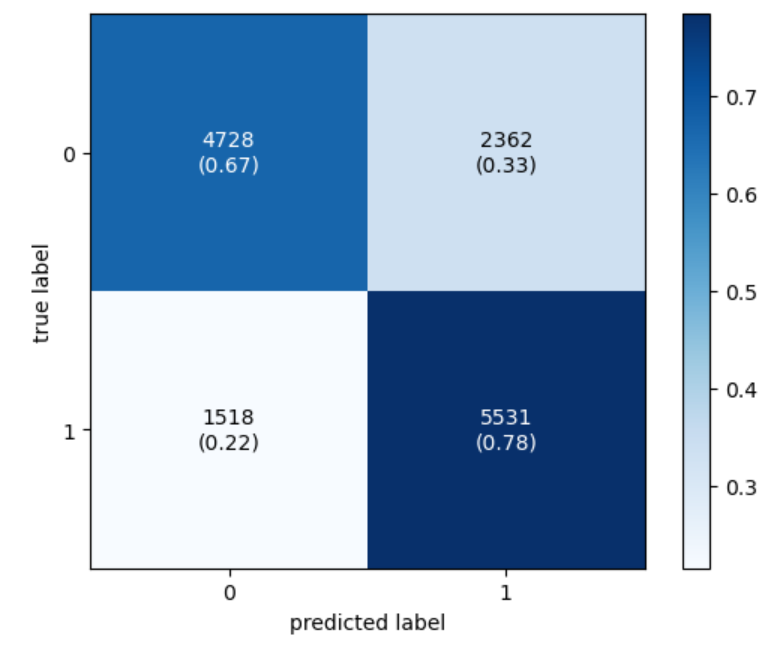
\includegraphics[width=0.3\textwidth]{knn_cm.png}
  \caption{KNN confusion matrix}
  \label{fig:knn}
\end{figure}

\subsection{SVM}
The fifth method we used is the SVM. We set the regularization parameter to C to be 1.0 and get the following confusion matrix and parameter weight graph:
\begin{figure}[H]
  \centering
  \begin{minipage}[b]{0.45\textwidth}
    \centering
    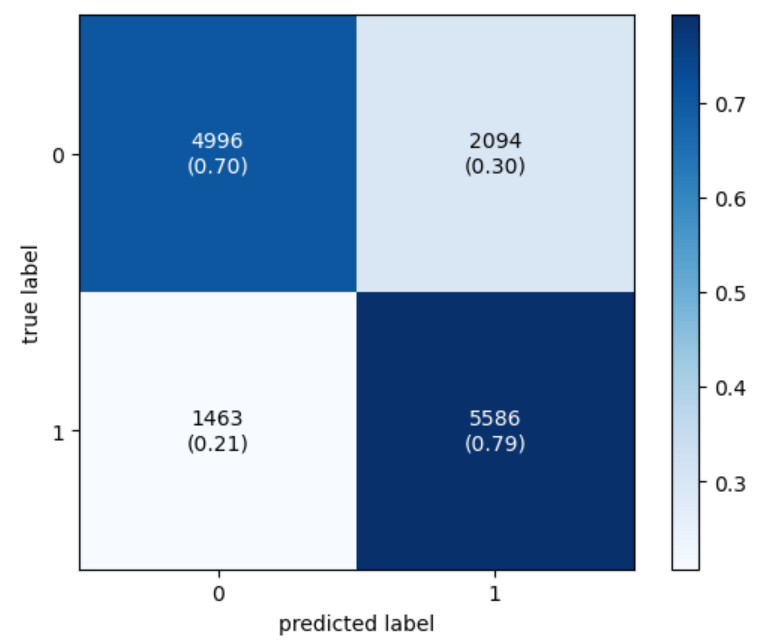
\includegraphics[width=0.7\linewidth]{svm_cm.png}
    \caption{SVM confusion matrix}
  \end{minipage}\hfill
  \begin{minipage}[b]{0.45\textwidth}
    \centering
    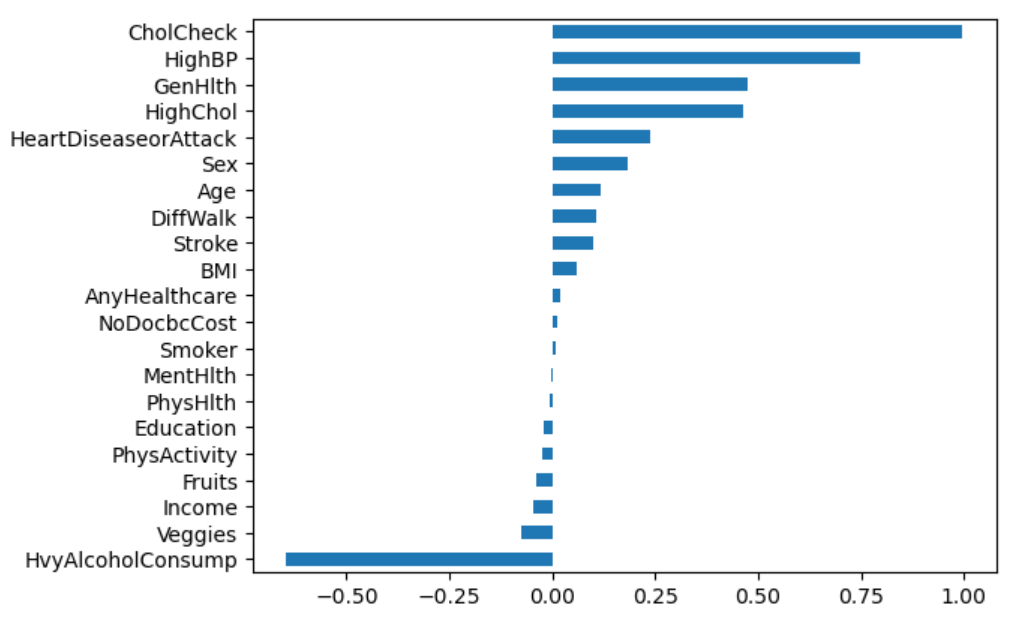
\includegraphics[width=0.7\linewidth]{svm_w.png}
    \caption{SVM feature importance}
  \end{minipage}
\end{figure}

\subsection{XGBoost}
In addition, we tried XGBoost, in which we set the learning rate to be 0.1. The following is confusion matrix and parameter weight graph:
\begin{figure}[H]
  \centering
  \begin{minipage}[b]{0.45\textwidth}
    \centering
    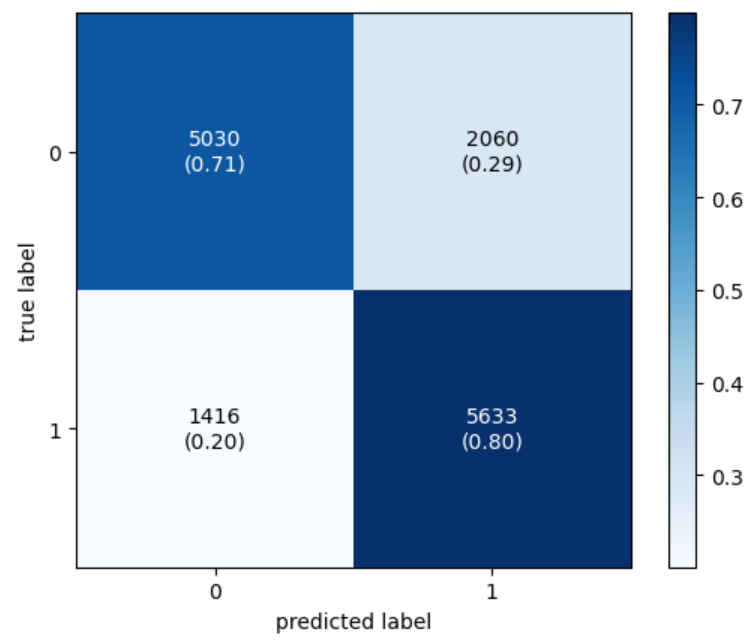
\includegraphics[width=0.7\linewidth]{xgboost_cm.png}
    \caption{XGBoost confusion matrix}
  \end{minipage}\hfill
  \begin{minipage}[b]{0.45\textwidth}
    \centering
    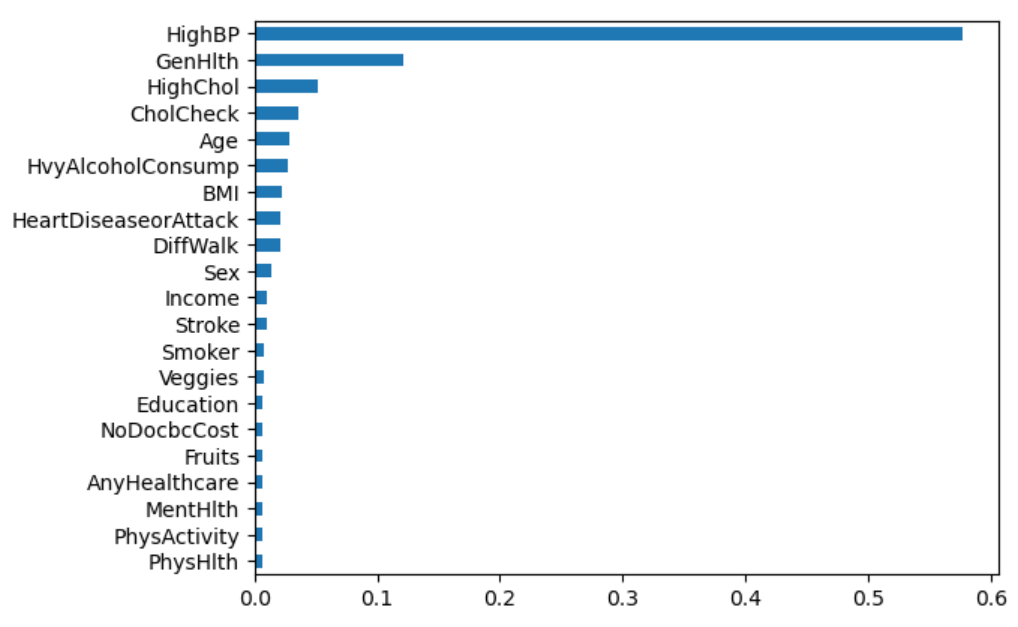
\includegraphics[width=0.7\linewidth]{xgboost_w.png}
    \caption{XGBoost feature importance}
  \end{minipage}
\end{figure}

\subsection{AdaBoost}
We performed hyperparametric tuning of the AdaBoost classifier. This involved using grid search to optimize three key parameters. After finding the optimal combination of parameters, we trained the AdaBoost model using these optimal settings on training data. Finally, we evaluated the performance of the optimized model on a test set.
\begin{figure}[H]
  \centering
  \begin{minipage}[b]{0.45\textwidth}
    \centering
    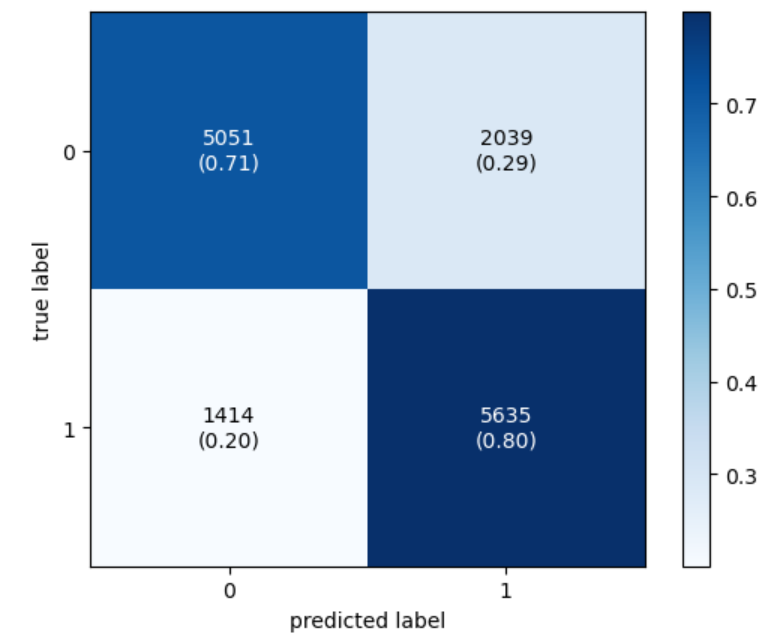
\includegraphics[width=0.7\linewidth]{adaboost_cm.png}
    \caption{AdaBoost confusion matrix}
  \end{minipage}\hfill
  \begin{minipage}[b]{0.45\textwidth}
    \centering
    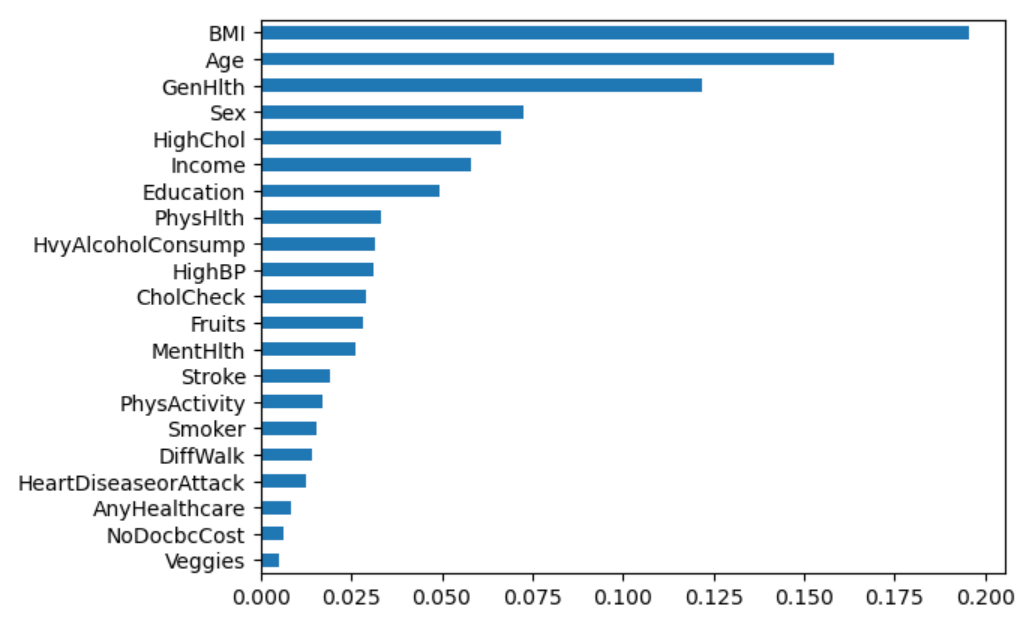
\includegraphics[width=0.7\linewidth]{adaboost_w.png}
    \caption{AdaBoost feature importance}
  \end{minipage}
\end{figure}

\section{Conclusion}

\subsection{Model Accuracy}
The combined accuracy of all models ranges from 0.72558 to 0.75536. AdaBoost surpasses other models in terms of both accuracy (0.75536) and F1 score (0.75502), making it the most compelling model in estimating diabetes. Its high-rate precision (0.75694) and recall (0.75536) indicate a balanced performance, which is essential for practical applications in the medical field. Despite AdaBoost's immensely competitive success, Random Forest and XGBoost also show respectable results, with XGBoost reaching the second highest F1 score. This suggests that ensemble methods, in general, are more effective for this application due to their ability to handle complex patterns and data imbalances better than simpler models like Logistic Regression. Likewise, KNN provided the worst results as this method does not handle datasets with many samples as well.
\begin{figure}[H]
  \centering
  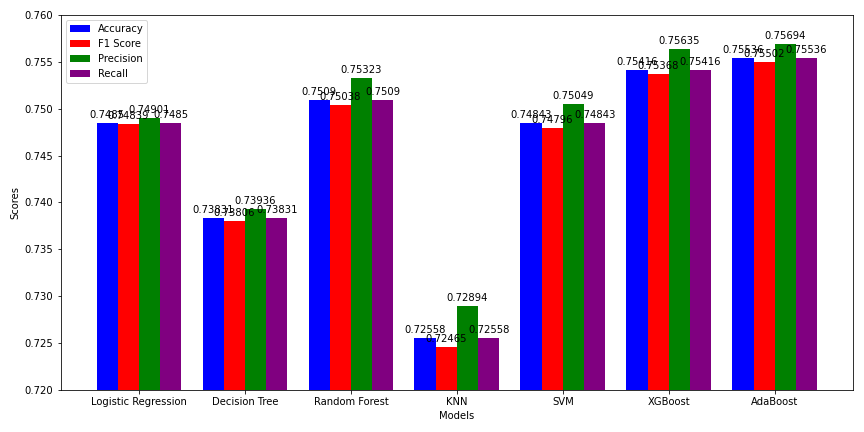
\includegraphics[width=0.8\textwidth]{combined.png}
  \caption{Accuracy, F1, precision, and recall values for each model}
  \label{fig:15}
\end{figure}
While measurements indicate that although AdaBoost is the most accurate and has the highest F1 score, the overall model misclassification error does not vary greatly or is very similar across all models. This suggests that improvements in model performance may also be obtained from further feature engineering or data preprocessing to reduce these errors.It is worth noting that two boosting methods perform better than other methods. The reason why boosting methods like AdaBoost and XGBoost often perform better, particularly in complex predictive tasks like diabetes prediction from survey data, can be attributed to several key characteristics of boosting algorithms. First, many traditional models like decision trees tend to overfit the data, showing high variance but low bias, whereas models like logistic regression may underfit, showing high bias but low variance. Boosting methods manage to balance bias and variance effectively. They build on top of weak models (typically high bias) and by focusing iteratively on reducing errors, they also manage to keep variance in check. Also, Boosting is designed to sequentially correct the mistakes of prior models and combine many weak learners (models that perform only slightly better than random guessing) to create a strong learner (Chen \& Guestrin, 2016). This approach effectively reduces both the bias (error due to erroneous assumptions in the learning algorithm) and variance (error from sensitivity to small fluctuations in the training set) of the model. In addition, according to Hastie et al. (2009) and Murphy (2012), boosting method can naturally process continuous and classified data, and can naturally process missing data. 

\subsection{Results and Analysis}
Examining the outcome with the two models that have the highest accuracy scores, we utilized feature importance plots from both the AdaBoost and XGBoost models to derive multiple inferences about the importance of different predictors in determining the likelihood of someone being diagnosed with diabetes.

In the XGBoost model, high blood pressure (HighBP) is the most influential variable,
indicating a strong association with diabetes. This factor is still important in the AdaBoost model but ranks slightly lower. 

The AdaBoost models, which place an emphasis on sex and body mass index as well as on their interactions, show the prediction that obesity and increased body mass index are strong predictors of increased diabetes risk. The AdaBoost model therefore revealed that these two factors markedly influence diabetes risk, and that by looking at sex as well as body mass index their combined effect on diabetes risk is certainly not simply additive.

The two models each individually and consistently identify Cholesterol Levels (HighChol) as well as General Health (GenHlth) as a factor for prediction. However, their orders of importance are different. This underscores the significance of lifestyle factors in diabetes risk, and Age shows up to be a significant factor in both models, as it should be since diabetes risk growth exponentially with age.
\pagebreak

\section{References}
\begin{hangparas}{.25in}{1}
Centers for Disease Control and Prevention. (2014, May 16). \textit{CDC - about BRFSS}. Centers for Disease Control and Prevention. \url{https://www.cdc.gov/brfss/about/index.htm} \\

Centers for Disease Control and Prevention. (2023a, May 8). \textit{Chronic disease center (NCCDPHP)}. Centers for Disease Control and Prevention. \url{https://www.cdc.gov/chronicdisease/index.htm} \\

Centers for Disease Control and Prevention. (2023b, September 5). \textit{What is diabetes?}. Centers for Disease Control and Prevention. \url{https://www.cdc.gov/diabetes/basics/diabetes.html} \\

Centers for Disease Control and Prevention. (2023c, November 29). \textit{National Diabetes Statistics Report}. Centers for Disease Control and Prevention. \url{https://www.cdc.gov/diabetes/data/statistics-report/index.html} \\

Chen, T. and Guestrin, C. (2016). Xgboost: A scalable tree boosting system. In Proceedings of the 22Nd ACM SIGKDD International Conference on Knowledge Discovery and Data Mining, KDD 16, pages 785–794, New York, NY, USA. \\

Hastie, T., Tibshirani, R., and Friedman, J. (2009). The Elements of Statistical Learning: Data Mining, Inference, and Prediction, Second Edition. Springer Series in Statistics. Springer. \\

Murphy, K. P. (2012). Machine Learning: A Probabilistic Perspective. The MIT Press. \\

Parker, E. D., Lin, J., Mahoney, T., Ume, N., Yang, G., Gabbay, R. A., ElSayed, N. A., \& Bannuru, R. R. (2024). Economic Costs of Diabetes in the U.S. in 2022. \textit{Diabetes care}, 47(1), 26–43. \url{https://doi.org/10.2337/dci23-0085} \\
\end{hangparas}

\end{document}
